% !TEX root = ../main.tex

\chapter{Methodik}
\label{cha:met}

Der volle Umfang diese Thesis setzt sich aus drei Unterprojekten zusammen, die als Gesamtheit eine Pipeline zum Trainieren eines neuronalen Netzes mit Inferenz auf echten Daten schafft. Im ersten Teil dieser Pipeline, \autoref{sec:met:data}, werden Daten zum Training des neuronalen Netzes erstellt. Diese Daten unterliegen der Voraussetzung, reale Aufnahmen von Dartscheiben zu simulieren, sodass ein neuronales Netz mit diesen trainiert werden kann. Der zweite Bauteil der Pipeline ist die algorithmische Normalisierung von Aufnahmen, \autoref{sec:met:cv}. Die Daten werden in diesem Schritt für die Inferenz mit dem neuronalen Netz vorbereitet. Dieser Schritt ist durch Verwendung klassischer \ac{CV} realisiert. Das letzte Teilprojekt dieser Thesis ist die Dartpfeil-Erkennung, \autoref{sec:met:ai}, in der die Dartpfeile in normalisierten Bildern lokalisiert werden. Durch diesen Schritt ist ein Scoring der erzielten Punktzahl möglich.

% -------------------------------------------------------------------------------------------------
\section{Datengenerierung}
\label{sec:met:data}

Die Datengrundlage für dieses Projekt setzt sich aus drei verschiedenen Quellen zusammen, eine dieser Quellen ist die synthetische Generierung realistischer Daten. Der Prozess der Datengenerierung wird in den folgenden Unterkapiteln erläutert.

\subsection{3D-Modellierung und Rendering}
\label{sec:met:data:model}

Die Simulation realer Aufnahmen zur Generierung realistischer Daten geschieht durch die Verwendung von 3D-Software zur Modellierung und Ray-Tracing zum Rendern von Aufnahmen. In der 3D-Software wird eine Szene erstellt, die relevante Objekte mit entsprechenden Materialien zur Verfügung stellt. In den folgenden Abschnitten wird auf die Art der Parametrisierung und die konkreten Objekte in der Szene eingegangen.

\subsubsection{Parametrisierung}
\label{sec:met:data:model:param}

Die Zusammensetzung, Geometrie und Texturierung der Objekte basiert auf Zufallsvariablen, die durch einen zufällig uniform gewählten Seed $s \in [0, s_{max}]$ bestimmt werden. Durch die Verwendung eines Seeds ist ein deterministisches Erstellen der Objekte möglich. In Abhängigkeit vom Seed wird ein Altersfaktors $a = \left( \frac{s}{s_{max}} \right)^k$ mit $k \in \mathbb{R}_{>0}$ bestimmt, dessen Magnitude den Grad der Abnutzung der unterschiedlichen Objekte der Szene zu bestimmen. Eine Visualisierung von $a$ in Abhängigkeit von $s$ ist in \autoref{fig:age} dargestellt. Ein hohes Alter der Dartscheibe äußert sich unter anderem durch Verfärbungen der Felder, geometrische Verformungen der Spinne und Risse im Sisal, bei Dartpfeilen bestimmt der Altersfaktor die Verformung der Flights. Für diese Arbeit wurde sich für einen Altersfaktor mit Exponent $k=5$ entschieden.

\begin{center}
    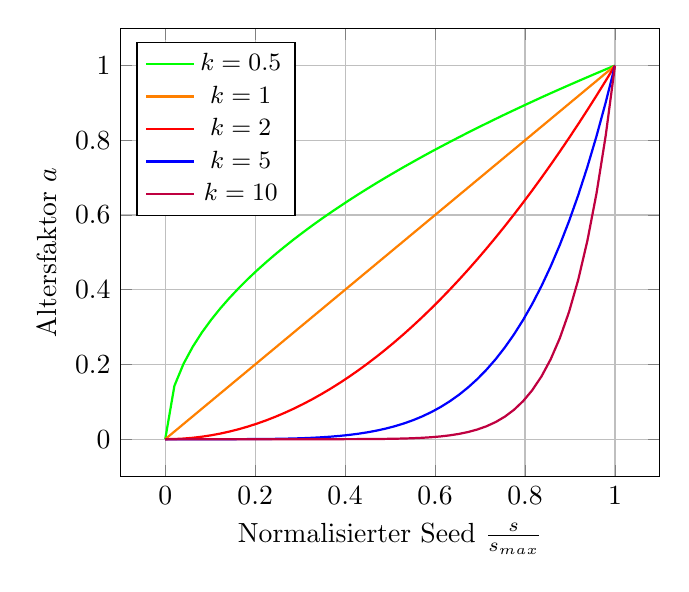
\begin{tikzpicture}
        \begin{axis}[
                ymin = -0.1,
                ymax=1.1,
                domain = 0:1,
                samples=50,
                xlabel={Normalisierter Seed $\frac{s}{s_{max}}$},
                ylabel={Altersfaktor $a$},
                scaled x ticks = false,
                grid=both,
                legend pos=north west,
                legend style={font=\small}
            ]
            \addplot[thick,green] {x^0.5};  \addlegendentry{$k=0.5$}
            \addplot[thick,orange]{x^1};    \addlegendentry{$k=1$}
            \addplot[thick,red]   {x^2};    \addlegendentry{$k=2$}
            \addplot[thick,blue]  {x^5};    \addlegendentry{$k=5$}
            \addplot[thick,purple]{x^10};   \addlegendentry{$k=10$}
        \end{axis}
    \end{tikzpicture}
    \captionof{figure}{Abhängigkeit des Altersfaktors $a$ von dem Seed $s$ für verschiedene Exponenten $k$.}
    \label{fig:age}
\end{center}

\subsubsection{Objekte in der Szene}
\label{sec:met:data:model:objects}

\subsubsection{Dartscheibe}
\label{sec:met:data:model:obejcts:board}

Die Dartscheibe ist das zentrale Objekt der Szene und damit wichtig für die Variabilität der Daten. Die Geometrie der Dartscheibe richtet sich nach dem Richtlinien \quotes{Playing and Tournament Rules} der \ac{WDF} \cite{wdf-rules}. In dem Regelwerk sind die Dimensionen und Abstände der Dartfelder, sowie etwaige Toleranzen festgelegt. In dieser Arbeit wurden alle Annahmen für Dartscheiben und -pfeile auf der Grundlage dieses Regelwerks getroffen. Starke Abweichungen durch esoterische Maße und Erscheinungsbilder, die nicht durch dieses Regelwerk gestützt sind, werden für diese Arbeit nicht in Betracht gezogen. Kleine Abweichungen dieser Standards durch hohe Altersfaktoren $a$ sind jedoch möglich.

Neben der Geometrie der Dartscheibe ist das Aussehen durch die Texturierung ein relevanter Aspekt des Objekts. Nicht nur muss das Material das Sisal der Felder und der umliegenden Scheibe realistisch abbilden, es muss zudem auch zu erwartende Umgebungseinflüsse auf Dartscheiben simulieren. Zentral sind dabei Abnutzungen in Form von Verfärbung der Felder, Einstichlöcher durch Dartpfeile und Risse im Sisal. Die Ausprägung dieser Gebrauchsspuren ist durch den Parameter $a$ moduliert.
Weiterhin sind neben diesen großen Adaptionen des Materials auch Details relevant, die durch Beobachtungen echter Dartscheiben aufgefallen sind. So sind beispielsweise Staubpartikel, kleine Haare und Kratzer auf dem Material relevante Details, die auf echten Dartscheiben identifiziert wurden und ebenfalls im Modell simuliert werden.

Alle diese Variabilitäten in den Dartscheiben sorgen für unterschiedliche Beschaffenheiten von Dartscheiben, die zufällig anhand eines Seeds generiert werden. Beispiele für simulierte Dartscheiben sind in \autoref{img:dartscheiben} gegeben. In der Abbildung sind drei Dartscheiben mit unterschiedlichen Altersfaktoren $a$ gegeben.

\begin{figure}
    \centering
    \begin{subfigure}{0.3\textwidth}
        \centering
        \includegraphics[width=\textwidth]{imgs/dartscheibe_a=0.png}
        \caption{$a=0$}
        \label{img:dartscheibe_neu}
    \end{subfigure}
    \hfill
    \begin{subfigure}{0.3\textwidth}
        \centering
        \includegraphics[width=\textwidth]{imgs/dartscheibe_a=0.5.png}
        \caption{$a\approx0.5$}
        \label{img:dartscheibe_mittel}
    \end{subfigure}
    \hfill
    \begin{subfigure}{0.3\textwidth}
        \centering
        \includegraphics[width=\textwidth]{imgs/dartscheibe_a=1.png}
        \caption{$a=1.0$}
        \label{img:dartscheibe_alt}
    \end{subfigure}
    \caption{Dartscheiben mit unterschiedlichen Altersfaktoren $a$.}
    \label{img:dartscheiben}
\end{figure}

% -------------------------------------------------------------------------------------------------
\section{Normalisierung mittels Computer Vision}
\label{sec:met:cv}

.

% -------------------------------------------------------------------------------------------------
\section{Dartpfeil-Erkennung}
\label{sec:met:ai}

.
